\section{Diskussion}
\label{sec:Diskussion}
Die Differenz zwischen dem berechneten $R_\text{eff}$ und dem in der Schaltung eingebauten Widerstand $R_\text{1}$ beträgt$\Delta R=60.1 \,\si{\ohm}$.
Diese lässt sich auf Innenwiderstand des Funktionengenerators von $R_{\mathrm{Generator}}=50\,\si{\ohm}$ zurückführen.
Daher wird, wie in der Auswertung erwähnt, der Generatorinnenwiderstand bei der Berechnung der Frequenzabhängigkeit der Kondensatorspannung berücksichtigt.
Die verbleibende Differenz $\Delta R-R_{\mathrm{Generator}}=10.1 \,\si{\ohm}$ lässt sich mit kleinen Messunsicherheiten -- also statistischen Fehlern -- begründen und liegt annähernd im Toleranzbereich.

Bei der Bestimmung des Dämpfungswiderstandes $R_{\mathrm{ap}}$ zeigt sich eine Abweichung
des experimentell bestimmten Wertes von $23\%$ zum Theoriewert. Dies lässt sich einerseits
auf das Vernachlässigen von den Innenwiderständen der weiteren Bauteile und
andererseits auf Schwierigkeiten beim Ablesen des Widerstandes zurückführen. Im Grenzbereich zeigten
sich keine erkennbaren Unterschiede im Verlauf der Kondensatorspannung.

Beim Vergleich der gemessenen beziehungsweise aus den Plots abgelesenen Messgrößen zeigen sich nur geringe Abweichungen gegenüber den Theoriewerten.
Im Detail zeigt ein Vergleich zwischen der theoretisch aus den Kenngrößen des Schwingkreises berechneten Güte $q_\mathrm{Theorie}$ mit der experimentell bestimmten Güte $q_\mathrm{Experiment}$ eine Abweichung von $8\%$.
Für die Breite der Resonanzkurve ergibt sich eine Abweichung von $5\%$.

Für die bestimmten Werte bei der Beobachtung der Phasenverschiebung in Abhängigkeit von der
Frequenz zeigt sich für $\omega_1$ und $\omega_{\mathrm{res}}$ eine Abweichung kleiner als $1\%$. Für $\omega_2$ erhält man selbige zu $4\%$.

Die abgelesenen Werte liegen alle absolut im Rahmen der Toleranz und sind auf statistische Fehler
und Ablesefehler zurückzuführen.

Allerdings fiel bereils zu Beginn der Messung auf, dass der Funktionengenerator keinen richtigen Nadelimpuls lieferte. Stattdessen lieferte der Generator einen Rechteckimpuls. Vergleiche dazu Abbildung \ref{fig:blabliblub}.
Wahrscheinlich wird dies allerdings wenig Einfluss auf die Messung gehabt haben.

Alle bestimmten Messgrößen finden sich in Tabelle \ref{tab:all_values}. Falls ein Theoriewert bestimmt wurde, ist zudem die prozentuale Abweichung zwischen Experiment und Theorie angegeben.
\begin{figure}
	\centering
	\caption{Spannungsverlauf der Generatorspannung bei eingestellter Nadelimpulsfunktion.}
	\label{fig:blabliblub}
	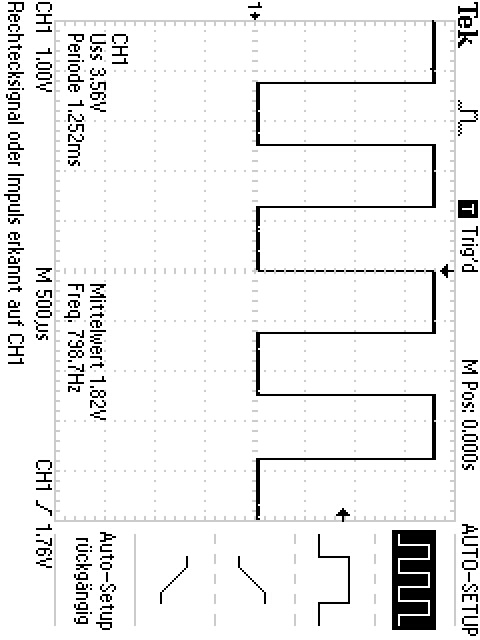
\includegraphics[width = 0.5 \textwidth, angle=90]{Bilder/a)rectangle/F0001TEK.JPG}
\end{figure}
\begin{table}
	\centering
	\caption{Tabelle aller bestimmen/abgelesenen Werte}
	\label{tab:all_values}
	\begin{tabular}{cccc}
		\toprule
		Messgröße                           & Experiment                                   & Theorie                                  & Abweichung \\
		\midrule
		Abklingdauer $T_{\text{ex}}$          & $(18.7 \pm 0.2) \cdot 10^{-5}\,\si{\second}$ & \--                                      & \--        \\
		Schaltungswiderstand $R_{\text{eff}}$ & (108.2 \pm 1.0) \,\si{\ohm}                  & \--                                      & \--        \\
		$R_{\text{ap}}$                       & \SI{3400}{\ohm}                              & (4390 \pm 9) \, \si{\ohm}                & $22.6\%$   \\
		Resonanzüberhöhung $q$              & 3.61                                         & (3.923 \pm 0.009)                        & $8\%$      \\
		$\omega_+ - \omega_-$                 & $9.25 \cdot 10^{3} \,\si{\Hz}$               & $(8.81\pm 0.03) \cdot 10^{3} \,\si{\Hz}$ & $5\%$      \\
		$\omega_{\mathrm{res}}$               & $33.7\cdot 10^{3} \,\si{\Hz}$                & $(34.0 \pm 0.1)\cdot 10^{3} \,\si{\Hz}$  & $0.9\%$    \\
		\bottomrule
	\end{tabular}
\end{table}
